% ============================================================================
% figures.tex — TikZ / pgfplots / booktabs source for the SimSpect writeup.
%
% Standalone: `pdflatex figures.tex` (needs tikz, pgfplots>=1.16, booktabs, xcolor,
% colortbl, geometry, amssymb). No TeX toolchain was available where this was
% written, so it is unverified-locally but uses only standard constructs — compile
% in your paper env and tweak sizes to taste. Every number matches
% paper_figures/make_paper_figures.py (provenance there) and PAPER_RESULTS.md.
%
% Contents (copy the snippet you want into the paper):
%   TBL-BUGS  the big bug table grouped by defense (provenance + who found it)
%   TBL-SCOPE the 8 AMuLeT bugs vs SimSpect's leakage model (F2)
%   TBL-SCORE the SimSpect scoreboard (F1c)
%   FIG-TARGET   test targeting 17% vs 100% (F3)
%   FIG-STALLS   stall-knob sensitivity (F4)
%   FIG-FRAG     fragility threshold (F5)
%   FIG-EFF      AMuLeT vs SimSpect efficiency (F8: detection + gem5-cost decomp)
%   FIG-RACE     the VP<->squash race schematic (F6)
%   FIG-RECON    the two recon gadgets (F7)
% ============================================================================
\documentclass[11pt]{article}
\usepackage[margin=1in,landscape]{geometry}
\usepackage{tikz,booktabs,xcolor,colortbl,amssymb}
\usepackage{pgfplots}
\pgfplotsset{compat=1.16}
\usepgfplotslibrary{groupplots}
\usetikzlibrary{positioning,arrows.meta,backgrounds,fit,shapes.geometric,calc}

% layer palette (matches the PNGs / bug/BUG_TAXONOMY.md)
\definecolor{ctarget}{HTML}{D62728}  % real defense bug
\definecolor{copen}{HTML}{E377C2}    % candidate / open
\definecolor{cchecker}{HTML}{FF7F0E} % checker artifact
\definecolor{calloy}{HTML}{1F77B4}   % alloy / model
\definecolor{cpipe}{HTML}{D4A017}    % pipeline
\definecolor{cclean}{HTML}{2CA02C}   % holds / SimSpect
\definecolor{camulet}{HTML}{8C564B}  % AMuLeT / out of scope
\newcommand{\s4}{\textcolor{ctarget}{$\blacksquare$}} % real
\newcommand{\rowgrp}[1]{\rowcolor{black!8}\multicolumn{6}{l}{\textbf{#1}}\\}

\begin{document}
\pagestyle{empty}

% ============================================================================
% TBL-BUGS — the big bug table grouped by defense
% ============================================================================
\begin{table}[p]\centering\small
\setlength{\tabcolsep}{5pt}\renewcommand{\arraystretch}{1.25}
\caption{Speculative-execution defense bugs, grouped by defense: where each was
first known, which tool exhibits it, whether it is in SimSpect's leakage model,
and the verdict. \textbf{Found-by:} \textcolor{cclean}{SimSpect} /
\textcolor{camulet}{AMuLeT} / \textbf{Both} / source-audit. Verdict:
\s4~real target bug $\cdot$ \textcolor{copen}{$\blacksquare$}~candidate/open.}
\label{tab:bugs}
\begin{tabular}{@{}p{2.4cm}p{4.5cm}p{3.1cm}p{3.0cm}cp{2.4cm}@{}}
\toprule
\textbf{Defense} & \textbf{Bug} & \textbf{First known from} & \textbf{Found by} &
\textbf{In scope?} & \textbf{Verdict} \\
\midrule
\rowgrp{Recon-STT \quad\textnormal{\textit{/work/gem5-recon-modded, scheme 2}}}
& OTB --- \texttt{getOldestTaint} keeps the oldest (not youngest) taint source
  & This work (\texttt{reconresults.md})
  & \textcolor{cclean}{SimSpect} (hand-crafted$^{1}$)
  & $\times$ gen-gap & \s4~real \\
& STL/SLF --- store-to-load forward bypasses the taint check
  & This work (\texttt{reconresults.md})
  & \textcolor{cclean}{\textbf{SimSpect, live}} (\texttt{inst-014912})
  & $\checkmark$ & \s4~real \\
\midrule
\rowgrp{STT \quad\textnormal{\textit{/work/stt $\cdot$ amulet STT\_AE}}}
& Visibility-point\,$\leftrightarrow$\,squash race (load channel)
  & This work (slow-comm)
  & \textcolor{cclean}{SimSpect, live} (timing-regime)
  & $\checkmark$ & \s4~real \\
& Implicit-channel (branch) defense structurally non-functional
  & This work (source audit$^{2}$)
  & \textcolor{cclean}{SimSpect} (source-audited)
  & $\sim$$^{3}$ & \s4~real (source) \\
& Tainted spec \emph{store} $\to$ D-TLB entry (KV3)
  & DOLMA (prior); reported by AMuLeT
  & \textcolor{camulet}{AMuLeT}
  & $\times$ store xmit & \s4~real (known) \\
\midrule
\rowgrp{SPT-Fence \quad\textnormal{\textit{/work/gem5-spt, DDIFT}}}
& Visibility-point\,$\leftrightarrow$\,squash race (= STT class)
  & This work
  & \textcolor{cclean}{SimSpect, live} (timing-regime)
  & $\checkmark$ & \textcolor{copen}{$\blacksquare$}~candidate \\
& \textit{(no independent SPT bug --- the rest are model over-approximation)}
  & --- & --- & --- & --- \\
\midrule
\rowgrp{InvisiSpec \quad\textnormal{\textit{amulet InvisiSpec\_AE}}}
& Spec-load L1D \emph{eviction} of a conflicting line (UV1)
  & AMuLeT (headline)
  & \textcolor{camulet}{AMuLeT}
  & $\times$ eviction & \s4~real \\
& Single-thread MSHR interference (UV2)
  & AMuLeT (ext.\ Behnia et al.)
  & \textcolor{camulet}{AMuLeT}
  & $\times$ MSHR & \s4~real \\
& L1I speculative fetch (KV1)
  & Known (InvisiSpec authors)
  & \textcolor{camulet}{AMuLeT}
  & $\times$ I-cache & \s4~real (known) \\
\midrule
\rowgrp{CleanupSpec \quad\textnormal{\textit{amulet CleanupSpec\_AE}}}
& Spec store not cleaned on squash (UV3)
  & AMuLeT & \textcolor{camulet}{AMuLeT}
  & $\times$ residue & \s4~real \\
& Cacheline-split request not cleaned (UV4)
  & AMuLeT & \textcolor{camulet}{AMuLeT}
  & $\times$ residue & \s4~real \\
& Over-cleaning evicts a non-spec line (UV5)
  & AMuLeT & \textcolor{camulet}{AMuLeT}
  & $\times$ final-state & \s4~real \\
\midrule
\rowgrp{SpecLFB \quad\textnormal{\textit{amulet SpecLFB\_AE}}}
& First speculative load left unprotected (UV6)
  & AMuLeT
  & \textbf{Both} (\textcolor{camulet}{AMuLeT} fuzz @\,t39; \textcolor{cclean}{SimSpect} @\,t6, 23\%)
  & $\checkmark$ & \s4~real \\
\bottomrule
\end{tabular}

\vspace{2pt}\footnotesize
$^{1}$ real bug, but the generator does not yet emit the \texttt{ld$\to$other$\to$xm}
precursor (enumeration-cap artifact C3); demonstrated hand-crafted.\quad
$^{2}$ the pending-squash sub-race was fixed upstream by N.\,Mosier (master only).\quad
$^{3}$ the live \texttt{br\_x} ``leaks'' were the \texttt{check\_br} FP (B2, fixed);
A3 is a real \emph{source-level} gap not yet shown as a live generated leak.\quad
(\,gem5 livelock at \texttt{commitToIEWDelay}$\geq$5 is a generic gem5 quirk, not a
defense bug.)
\end{table}


% ============================================================================
% TBL-SCOPE — the 8 AMuLeT bugs vs SimSpect's leakage model  (F2)
% ============================================================================
\begin{table}[p]\centering\small
\renewcommand{\arraystretch}{1.2}
\caption{The 8 bugs AMuLeT reports on these defenses vs.\ SimSpect's leakage model.
SimSpect sees a leak iff it is the \emph{transmitter's own} access \emph{inside} the
speculative window. One is in scope: SpecLFB UV6.}
\label{tab:scope}
\begin{tabular}{@{}llll c@{}}
\toprule
\textbf{Bug} & \textbf{Defense} & \textbf{Leakage channel} & \textbf{Reason} & \textbf{Scope}\\
\midrule
UV1 & InvisiSpec & spec-load L1D eviction & Ruby eviction, not a transmitter access & \textcolor{camulet}{out}\\
UV2 & InvisiSpec & MSHR contention (timing) & shared resource; needs input-diff & \textcolor{camulet}{out}\\
KV1 & InvisiSpec & L1I spec fetch & I-cache state & \textcolor{camulet}{out}\\
UV3 & CleanupSpec & post-squash L1D residue & install is by-design; final-state diff & \textcolor{camulet}{out}\\
UV4 & CleanupSpec & split-request residue & final-state diff & \textcolor{camulet}{out}\\
UV5 & CleanupSpec & over-cleaning evicts NSL & final-state diff & \textcolor{camulet}{out}\\
KV3 & STT & tainted spec \emph{store} $\to$ D-TLB & store xmit + TLB (not in \texttt{leakage\_function}) & \textcolor{camulet}{out}\\
\rowcolor{ctarget!12}
\textbf{UV6} & \textbf{SpecLFB} & first spec \emph{load} installs a line & the transmitter's own in-window cache touch & \textcolor{ctarget}{\textbf{IN}}\\
\bottomrule
\end{tabular}
\end{table}


% ============================================================================
% TBL-SCORE — SimSpect scoreboard (F1c)
% ============================================================================
\begin{table}[p]\centering\small
\renewcommand{\arraystretch}{1.2}
\caption{SimSpect per-run scoreboard: raw hits collapse to confirmed real defense
bugs once model over-approximation and checker artifacts are filtered.}
\label{tab:score}
\begin{tabular}{@{}lrrrrl@{}}
\toprule
\textbf{Run} & \textbf{raw hits} & \textbf{model arti.} & \textbf{checker FP} & \textbf{candidate} & \textbf{REAL bug}\\
\midrule
Recon-STT (stock)        & 184    & ---    & 183  & 0     & \textcolor{ctarget}{\textbf{1 (SLF/A2)}}\\
STT (stock)              & 0      & ---    & ---  & ---   & 0 --- holds\\
STT (slow-comm)          & 23{,}988 & ---  & 21   & 4{,}122 & \textcolor{ctarget}{\textbf{19{,}845 (A4)}}\\
SPT-Fence (stock)        & 6{,}118 & 6{,}111 & 7   & 0     & 0\\
SPT-Fence (slow-comm)    & 77{,}555 & 73{,}158 & --- & 4{,}397 & 0$^{*}$ (A5 open)\\
\bottomrule
\end{tabular}

\vspace{1pt}\footnotesize $^{*}$the slow-comm \textsc{new} bucket contains the
$\sim$983 VP$\leftrightarrow$squash-race candidates shared with STT.
\end{table}


% ============================================================================
% FIG-TARGET — test targeting 17% vs 100%  (F3)
% ============================================================================
\begin{figure}[p]\centering
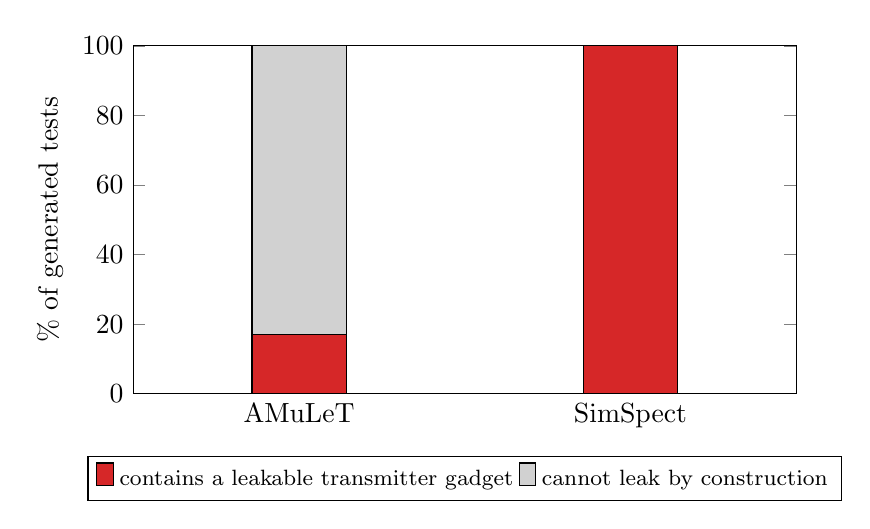
\begin{tikzpicture}
\begin{axis}[
  ybar stacked, width=10cm, height=6cm, bar width=34pt,
  symbolic x coords={AMuLeT, SimSpect}, xtick=data,
  ymin=0, ymax=100, ylabel={\% of generated tests},
  xticklabel style={align=center}, enlarge x limits=0.5,
  legend style={at={(0.5,-0.18)},anchor=north,legend columns=2,font=\footnotesize},
  nodes near coords={}, every node near coord/.append style={font=\footnotesize}]
\addplot[fill=ctarget] coordinates {(AMuLeT,17) (SimSpect,100)};
\addplot[fill=black!18] coordinates {(AMuLeT,83) (SimSpect,0)};
\legend{contains a leakable transmitter gadget, cannot leak by construction}
\node[white,font=\bfseries] at (axis cs:AMuLeT,8.5) {17\%};
\node[white,font=\bfseries] at (axis cs:SimSpect,50) {100\%};
\end{axis}
\end{tikzpicture}
\caption{Test targeting. Of AMuLeT's 500 random STT tests only 85 (17\%) contain a
window-valid speculative gadget (static analysis, \texttt{stt\_corpus\_gadgets.json});
100\% of SimSpect's 100{,}000 do, by the \texttt{tag\_xm} construction.}
\label{fig:target}
\end{figure}


% ============================================================================
% FIG-STALLS — stall-knob sensitivity @ commitToIEWDelay=3  (F4)
% ============================================================================
\begin{figure}[p]\centering
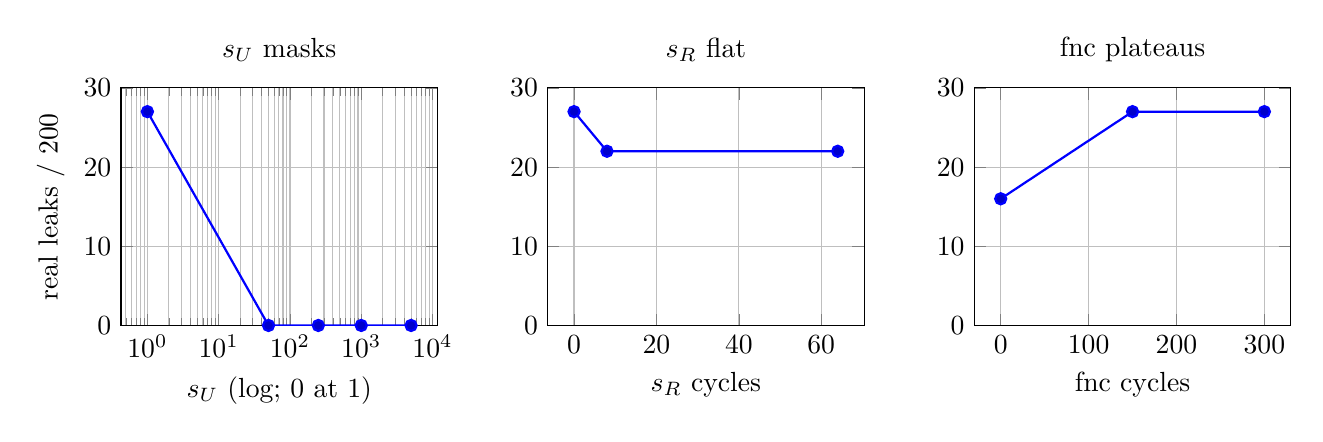
\begin{tikzpicture}
\begin{groupplot}[group style={group size=3 by 1,horizontal sep=1.4cm},
  width=5.6cm,height=4.6cm,ymin=0,ymax=30,grid=both,
  every axis plot/.append style={ctarget,thick,mark=*,mark options={solid}}]
\nextgroupplot[xmode=log,log basis x=10,xlabel={$s_U$ (log; 0 at 1)},
  title={$s_U$ masks},ylabel={real leaks / 200}]
\addplot coordinates {(1,27) (50,0.01) (250,0.01) (1000,0.01) (5000,0.01)};
\nextgroupplot[xlabel={$s_R$ cycles},title={$s_R$ flat}]
\addplot coordinates {(0,27) (8,22) (64,22)};
\nextgroupplot[xlabel={fnc cycles},title={fnc plateaus}]
\addplot coordinates {(0,16) (150,27) (300,27)};
\end{groupplot}
\end{tikzpicture}
\caption{Stall-knob sensitivity (STT @ \texttt{commitToIEWDelay}=3; 100\%
bucket-confirmed VP$\leftrightarrow$squash race). Only the window knob $s_U$ flips the
verdict, and it \emph{masks} (never manufactures): $s_U{\geq}50\to0$. $s_R$ is a flat
plateau; the leak survives \texttt{fnc}=0. \texttt{paper\_stalls/stt\_*/summary.json}.}
\label{fig:stalls}
\end{figure}


% ============================================================================
% FIG-FRAG — fragility threshold  (F5)
% ============================================================================
\begin{figure}[p]\centering
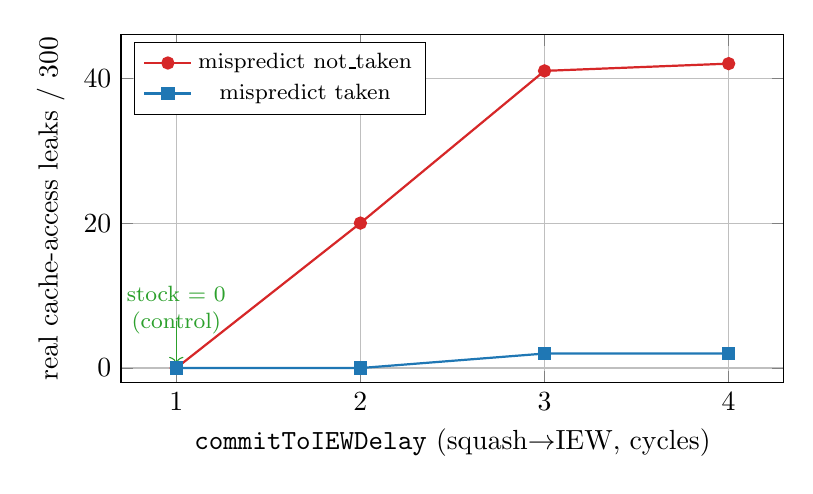
\begin{tikzpicture}
\begin{axis}[width=10cm,height=6cm,xlabel={\texttt{commitToIEWDelay} (squash$\to$IEW, cycles)},
  ylabel={real cache-access leaks / 300}, xtick={1,2,3,4}, ymin=-2,ymax=46,grid=both,
  legend style={at={(0.02,0.98)},anchor=north west,font=\footnotesize}]
\addplot[ctarget,thick,mark=*] coordinates {(1,0) (2,20) (3,41) (4,42)};
\addplot[calloy,thick,mark=square*] coordinates {(1,0) (2,0) (3,2) (4,2)};
\legend{mispredict not\_taken, mispredict taken}
\node[cclean,font=\footnotesize,align=center] at (axis cs:1,8)
  {stock = 0\\(control)};
\draw[cclean,->] (axis cs:1,6.5) -- (axis cs:1,0.6);
\end{axis}
\end{tikzpicture}
\caption{STT fragility threshold. Secure at stock (\texttt{commitToIEWDelay}=1, 0
leaks); leaks from $\geq2$. The Fence control's raw cache-reach is const-addr
over-approximation (tainted-address race $0/230$ at stock), so the real-leak control
is $0$. \texttt{paper\_fragility/frag\_d*}.}
\label{fig:frag}
\end{figure}


% ============================================================================
% FIG-EFF — AMuLeT vs SimSpect efficiency on the SpecLFB build  (F8)
% ============================================================================
\begin{figure}[p]\centering
% (left) detection: tests to first UV6
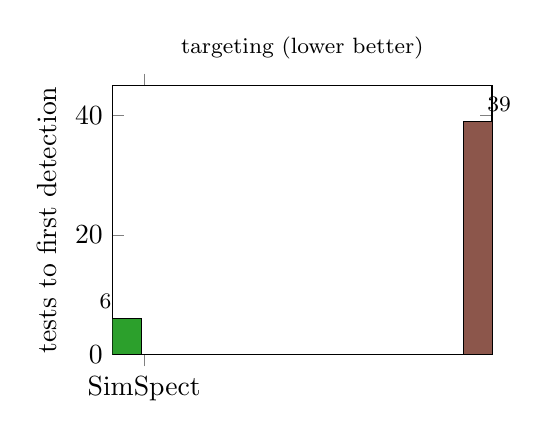
\begin{tikzpicture}
\begin{axis}[ybar,width=6.4cm,height=5cm,bar width=26pt,
  symbolic x coords={SimSpect,AMuLeT},xtick=data,ymin=0,ymax=45,
  ylabel={tests to first detection},nodes near coords,
  every node near coord/.append style={font=\footnotesize\bfseries},
  title={\footnotesize targeting (lower better)}]
\addplot[fill=cclean] coordinates {(SimSpect,6)}; \addplot[fill=camulet] coordinates {(AMuLeT,39)};
\end{axis}
\end{tikzpicture}\hfill
% (right) gem5-cost decomposition: only the sim core is comparable
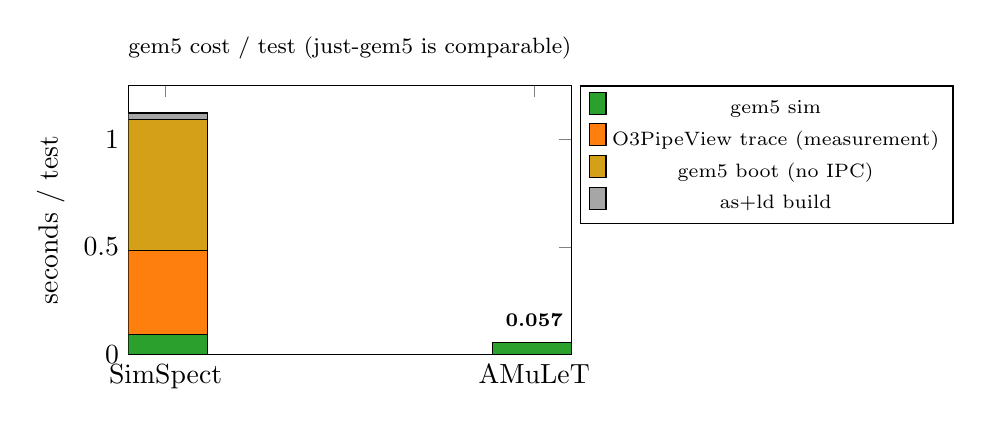
\begin{tikzpicture}
\begin{axis}[ybar stacked,width=7.2cm,height=5cm,bar width=30pt,
  symbolic x coords={SimSpect,AMuLeT},xtick=data,ymin=0,ymax=1.25,
  ylabel={seconds / test},
  legend style={at={(1.02,1)},anchor=north west,font=\scriptsize},
  title={\footnotesize gem5 cost / test (just-gem5 is comparable)}]
\addplot[fill=cclean]  coordinates {(SimSpect,0.092) (AMuLeT,0.057)};
\addplot[fill=cchecker]coordinates {(SimSpect,0.39)  (AMuLeT,0)};
\addplot[fill=cpipe]   coordinates {(SimSpect,0.61)  (AMuLeT,0)};
\addplot[fill=black!35] coordinates {(SimSpect,0.03) (AMuLeT,0)};
\legend{gem5 sim, O3PipeView trace (measurement), gem5 boot (no IPC), as+ld build}
\node[font=\scriptsize\bfseries] at (axis cs:AMuLeT,0.16) {0.057};
\node[white,font=\scriptsize\bfseries] at (axis cs:SimSpect,0.046) {0.092};
\end{axis}
\end{tikzpicture}
\caption{Efficiency on the SpecLFB build (UV6), measured. \textbf{Left:} SimSpect
flags UV6 at test \#6 vs AMuLeT's first contract violation at \#39 ($6.5\times$ fewer;
23\% vs 3.3\% density). \textbf{Right:} isolating \emph{just the gem5 time}, the
simulation cost is comparable (0.092 vs 0.057\,s/test); SimSpect's extra per-test cost
is the O3PipeView measurement trace + fresh gem5 boot (both harness/instrumentation),
not gem5 work. \texttt{results/STT\_6\_speclfb/amulet\_compare/fuzz.log},
\texttt{time\_gem5\_only.py}.}
\label{fig:eff}
\end{figure}


% ============================================================================
% FIG-RACE — the VP<->squash race schematic  (F6)
% ============================================================================
\begin{figure}[p]\centering
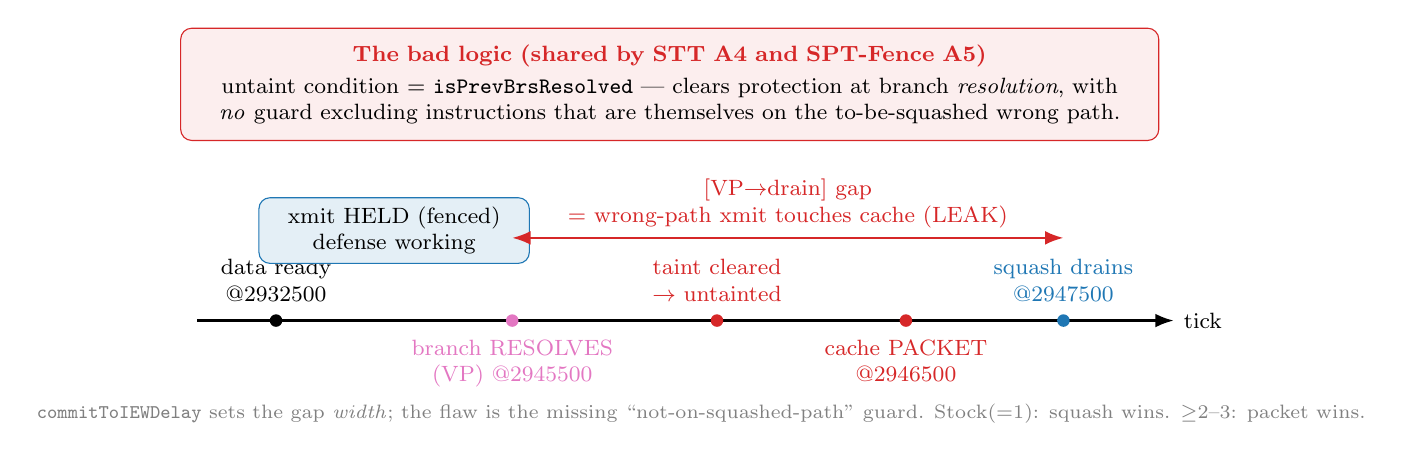
\begin{tikzpicture}[font=\footnotesize,>=Latex,
  ev/.style={circle,fill=#1,inner sep=1.6pt}]
% logic box
\node[draw=ctarget,fill=ctarget!8,rounded corners,text width=12cm,align=center,inner sep=6pt]
  (logic) at (0,3.0) {\textbf{\textcolor{ctarget}{The bad logic (shared by STT A4 and SPT-Fence A5)}}\\[2pt]
  untaint condition $=$ \texttt{isPrevBrsResolved} --- clears protection at branch
  \emph{resolution}, with \emph{no} guard excluding instructions that are themselves
  on the to-be-squashed wrong path.};
% timeline
\draw[->,thick] (-6,0) -- (6.4,0) node[right]{tick};
\node[ev=black]   (d) at (-5,0) {}; \node[above=1pt of d,align=center]{data ready\\@2932500};
\node[ev=copen]   (v) at (-2,0) {}; \node[below=1pt of v,align=center,copen]{branch RESOLVES\\(VP) @2945500};
\node[ev=ctarget] (t) at (0.6,0){}; \node[above=1pt of t,align=center,ctarget]{taint cleared\\$\to$ untainted};
\node[ev=ctarget] (p) at (3,0)  {}; \node[below=1pt of p,align=center,ctarget]{cache PACKET\\@2946500};
\node[ev=calloy]  (s) at (5,0)  {}; \node[above=1pt of s,align=center,calloy]{squash drains\\@2947500};
% held + gap
\node[draw=calloy,fill=calloy!12,rounded corners,above=18pt of d,xshift=1.5cm,text width=3.2cm,align=center]
  {xmit HELD (fenced)\\defense working};
\draw[<->,ctarget,thick] (-2,1.05) -- node[above,ctarget,align=center]{[VP$\to$drain] gap\\= wrong-path xmit touches cache (LEAK)} (5,1.05);
\node[below=24pt of d,xshift=5.4cm,gray,font=\scriptsize,align=center]
  {\texttt{commitToIEWDelay} sets the gap \emph{width}; the flaw is the missing
  ``not-on-squashed-path'' guard. Stock(=1): squash wins. $\geq$2--3: packet wins.};
\end{tikzpicture}
\caption{The visibility-point\,$\leftrightarrow$\,squash race (STT $=$ SPT-Fence): a
logic flaw whose exposure window is sized by \texttt{commitToIEWDelay}.}
\label{fig:race}
\end{figure}


% ============================================================================
% FIG-RECON — the two recon gadgets  (F7)
% ============================================================================
\begin{figure}[p]\centering
\begin{tikzpicture}[font=\scriptsize,>=Latex,node distance=5pt,
  b/.style={draw,rounded corners,fill=#1,text width=4.0cm,align=center,inner sep=3pt},
  x/.style={b=ctarget!85,text=white}]
% --- OTB (left) ---
\begin{scope}
\node[b=black!8] (o0) {branch\_outer (resolves FIRST, correctly not-taken)};
\node[b=calloy!18,below=14pt of o0,xshift=-2.2cm] (la) {load\_A $\to$ \%rax (older, tainted)};
\node[b=calloy!18,right=10pt of la] (lb) {load\_B $\to$ \%rcx (younger, still spec)};
\node[b=copen!50,below=14pt of la,xshift=2.2cm] (alu) {\texttt{leaq (\%rax,\%rcx)}: \texttt{getOldestTaint} keeps load\_A only};
\node[b=ctarget!12,below=8pt of alu] (fr) {branch\_outer resolves $\to$ \texttt{freeTaints} drops \%rax (load\_B still spec!)};
\node[x,below=8pt of fr] (xm) {\texttt{movq (\%rcx,\%rax)} XMIT: ``untainted'' addr $\to$ cache};
\draw[->](o0)--(la); \draw[->](o0)--(lb); \draw[->](la)--(alu); \draw[->](lb)--(alu);
\draw[->](alu)--(fr); \draw[->](fr)--(xm);
\node[above=2pt of o0,ctarget,font=\bfseries\scriptsize]{A1 --- OTB (\texttt{getOldestTaint})};
\end{scope}
% --- STL (right) ---
\begin{scope}[xshift=8.4cm]
\node[b=black!8] (s0) {\texttt{je end} --- MISPREDICT $\to$ spec window opens};
\node[b=calloy!18,below=12pt of s0] (sl) {\texttt{movq (\%rsi),\%rax} $\to$ \%rax TAINTED};
\node[b=cpipe!25,below=10pt of sl] (st) {\texttt{movq \%r8,(\%rsi,\%rax)} store to tainted addr};
\node[x,below=10pt of st] (sx) {\texttt{movq (\%rsi,\%rax),\%r10} XMIT: LSQ forwards $\to$ \texttt{NoFault} BEFORE the taint check};
\draw[->](s0)--(sl); \draw[->](sl)--(st); \draw[->](st)--(sx);
\node[below=6pt of sx,align=center,ctarget]{completes (ready-in-ROB @2682500)\\before squash @2683500, no cache packet};
\node[above=2pt of s0,ctarget,font=\bfseries\scriptsize]{A2 --- STL/SLF (store-forward bypass), caught LIVE};
\end{scope}
\end{tikzpicture}
\caption{The two recon STT taint-tracker bugs. A1 (OTB) is real but generator-unreachable
(C3, hand-crafted); A2 (STL/SLF) was caught live from generator output (\texttt{inst-014912}).}
\label{fig:recon}
\end{figure}

\end{document}
